\documentclass[UTF8,a4paper,12pt]{ctexart}

\usepackage[margin=2.54cm]{geometry}
\usepackage{setspace}
\usepackage{graphicx}
\usepackage[table]{xcolor}
\usepackage{tcolorbox}
\tcbuselibrary{skins}
\usepackage{booktabs}
\usepackage{array}
\usepackage{longtable}
\usepackage{tabularx}
\usepackage{float}
\usepackage{caption}
\usepackage{enumitem}
\usepackage{fancyhdr}
\usepackage{titlesec}
\usepackage{hyperref}
\usepackage{amsmath}
\usepackage{amssymb}
\usepackage{zhnumber}

% --- Google Material Design Colors ---
\definecolor{GoogleBlue}{HTML}{1A73E8}
\definecolor{GoogleGray}{HTML}{F8F9FA}
\definecolor{GoogleBorder}{HTML}{DADCE0}
\definecolor{GoogleText}{HTML}{202124}
\definecolor{GoogleHeader}{HTML}{F1F3F4}

\hypersetup{
  colorlinks=true,
  linkcolor=GoogleBlue,
  urlcolor=GoogleBlue,
  citecolor=GoogleBlue,
  pdftitle={分布式MiniSQL系统模块实现与测试报告},
  pdfauthor={请填写姓名}
}

% --- Web Typography (Sans-serif) ---
\renewcommand{\familydefault}{\sfdefault}
\setstretch{1.5}
\setlength{\parindent}{2em}
\setlength{\parskip}{0.5em}
\captionsetup{font=small, labelfont={color=GoogleBlue, bf}}
\setlist[enumerate]{label=\arabic*., leftmargin=2.8em, itemsep=0pt}
\setlist[itemize]{label=\textcolor{GoogleBlue}{\textbullet}, leftmargin=2.8em, itemsep=0pt}

\pagestyle{fancy}
\fancyhf{}
\cfoot{\textcolor{GoogleBorder}{\rule{0.5\textwidth}{0.4pt}}\\\vspace{0.2em}\thepage}
\renewcommand{\headrulewidth}{0pt}

\renewcommand{\thesection}{\arabic{section}}
\renewcommand{\thesubsection}{\arabic{section}.\arabic{subsection}}
\renewcommand{\thesubsubsection}{\arabic{section}.\arabic{subsection}.\arabic{subsubsection}}

% --- Modern Headings ---
\titleformat{\section}{\sffamily\zihao{3}\bfseries\color{GoogleBlue}}{\thesection}{0.5em}{}
\titleformat{\subsection}{\sffamily\zihao{4}\bfseries\color{GoogleText}}{\thesubsection}{0.5em}{}
\titleformat{\subsubsection}{\sffamily\zihao{-4}\bfseries\color{GoogleText}}{\thesubsubsection}{0.5em}{}

\titlespacing*{\section}{0pt}{1.2em}{0.6em}
\titlespacing*{\subsection}{0pt}{1em}{0.4em}
\titlespacing*{\subsubsection}{0pt}{0.8em}{0.3em}

\newcommand{\studentName}{请填写姓名}
\newcommand{\collegeName}{请填写学院}
\newcommand{\departmentName}{请填写系别}
\newcommand{\majorName}{请填写专业}
\newcommand{\studentId}{请填写学号}
\newcommand{\reportYear}{2026}
\newcommand{\reportMonth}{5}
\newcommand{\reportDay}{1}

\newcommand{\languageName}{Go}
\newcommand{\platformName}{macOS / Linux}
\newcommand{\moduleA}{Raft复制与存储}
\newcommand{\moduleB}{分片路由与协调}
\newcommand{\moduleC}{控制平面与API}

\newcommand{\coverline}[2]{#1 & \underline{\makebox[8cm][c]{#2}} \\[1.1em]}

\begin{document}

\begin{titlepage}
  \centering
  \vspace*{2.6cm}

  {\zihao{2}\bfseries 大规模信息系统构建技术导论\par}
  \vspace{2cm}
  {\zihao{-1}\bfseries 分布式MiniSQL系统模块实现与测试报告\par}

  \vfill

  \renewcommand{\arraystretch}{1.4}
  \begin{tabular}{>{\zihao{4}}p{2.8cm} >{\zihao{4}}p{9cm}}
    \coverline{姓名：}{\studentName}
    \coverline{学院：}{\collegeName}
    \coverline{系：}{\departmentName}
    \coverline{专业：}{\majorName}
    \coverline{学号：}{\studentId}
  \end{tabular}

  \vfill

  {\zihao{4}\reportYear~年~\reportMonth~月~\reportDay~日\par}
\end{titlepage}

\pagenumbering{arabic}
\setcounter{page}{1}

\tableofcontents
\clearpage

\zihao{-4}

\section{项目背景与业界架构对比}
\subsection{分布式数据库演进背景}
随着业务规模的高速增长，传统关系型数据库依赖纵向扩展（Scale-up）的模式已无法满足海量数据与高并发的读写需求；而传统 NoSQL 数据库虽然实现了水平扩展（Scale-out），但往往以牺牲 ACID 事务和强一致性（通常仅保证最终一致性）为代价。现代分布式数据库（如 Google Spanner、TiDB/TiKV 等）致力于在提供近乎无限的横向扩缩能力的同时，依然保持强事务一致性和高可用性。本分布式 MiniSQL 系统正是在这一背景下，借鉴工业界主流分布式架构设计思想的轻量级实现。

\subsection{业界典型架构分析}
\subsubsection{Google Spanner}
Google Spanner 是业界最具代表性的可横向扩展强一致关系型数据库之一\cite{spanner-paper}。正如 Google Cloud 官方文档所述：“Spanner 确保强事务一致性，这意味着无论数据的大小或分布如何，每次读取都将反映最新的更新”\cite{spanner-docs}。如图\ref{fig:spanner-arch}所示，Spanner 采用了计算与存储分离的架构，底层数据会自动“分块”（Splits）以实现横向扩展。它利用 Paxos 同步架构保证数据的高可用性与跨区域复制，并创新性地使用 TrueTime 分布式时钟来实现强 ACID 事务隔离。Spanner 能够提供高达 99.999\% 的可用性（SLA承诺），是现代云原生分布式数据库的重要代表。

\begin{figure}[H]
  \centering
  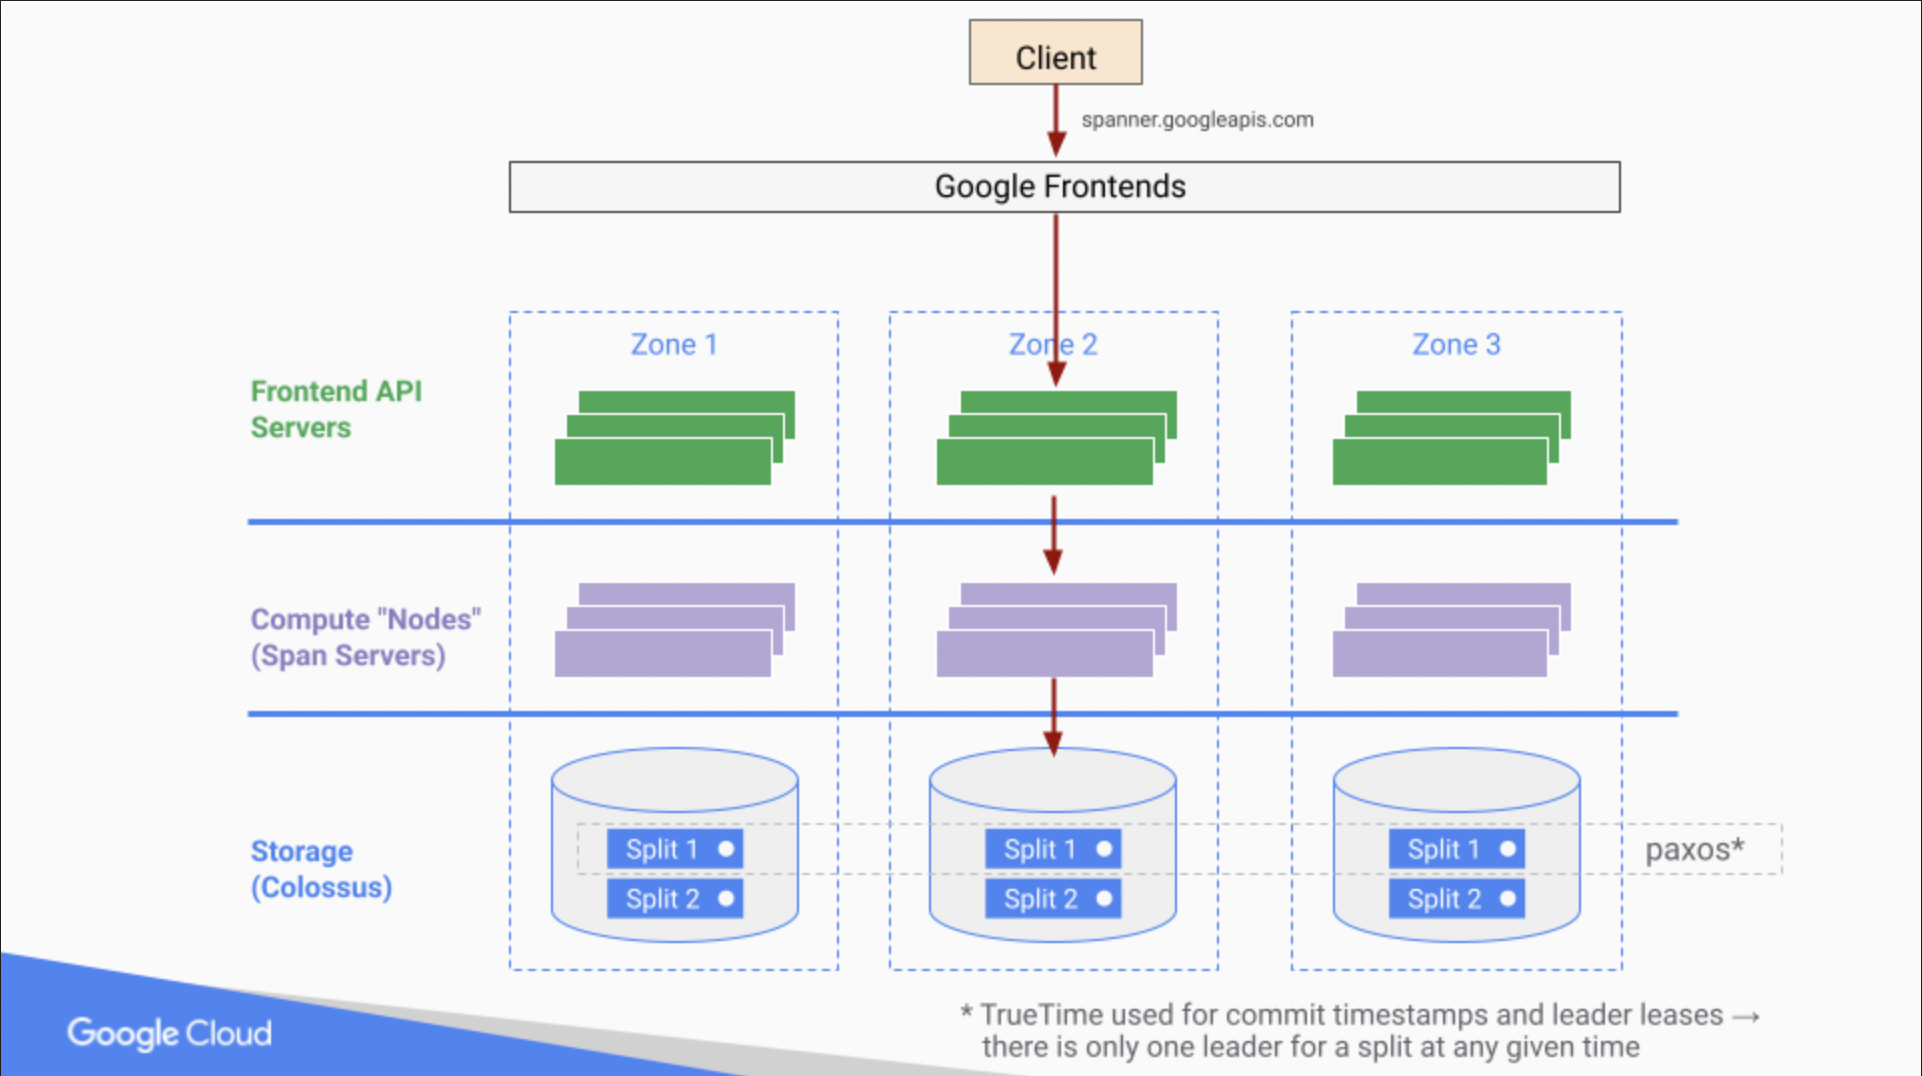
\includegraphics[width=0.85\textwidth]{spanner_arch.png}
  \caption{Google Spanner 架构示意图}
  \label{fig:spanner-arch}
\end{figure}

\subsubsection{TiKV}
TiKV 是另一个广泛应用的开源分布式事务键值数据库\cite{tikv-docs}，常作为 TiDB 的底层存储引擎。官方将其定义为“一个支持 ACID 事务的分布式 KV 存储引擎，旨在提供极高的数据可靠性与线性一致性”。如图\ref{fig:tikv-arch}所示，TiKV 采用了基于 Region 的 Multi-Raft 架构。数据被划分为多个独立的分片（Region），每个 Region 作为一个单独的 Raft 副本组分布在不同的节点上，底层依托 RocksDB 进行数据持久化。这种设计使得 TiKV 具备极高的水平扩展能力与细粒度的负载均衡特性；在典型部署中，业务请求通常先经过 TiDB，再由 TiDB 将请求路由到对应 Region Leader 所在的 TiKV 节点。

\begin{figure}[H]
  \centering
  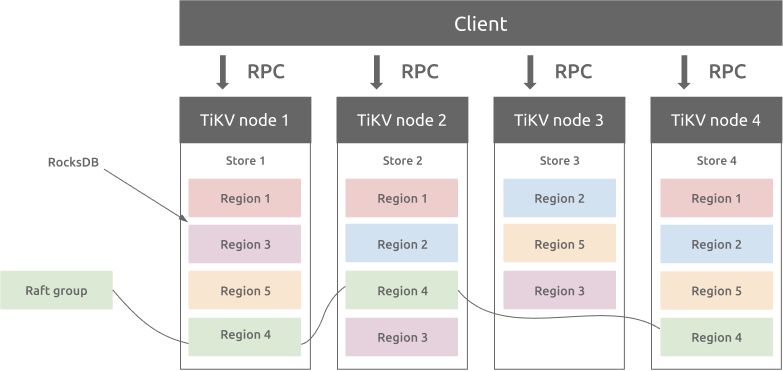
\includegraphics[width=0.85\textwidth]{tikv-arch.png}
  \caption{TiKV Multi-Raft 架构示意图}
  \label{fig:tikv-arch}
\end{figure}

\subsection{本系统架构定位}
本分布式 MiniSQL 系统（DDB）在设计上深度借鉴了 Spanner 与 TiKV 的核心思想。系统同样实现了计算层（SQL 解析与协调路由）与存储层（共识复制与本地存储）的解耦，底层依托 Raft 共识算法保证数据的多副本强一致性，并使用嵌入式引擎 BoltDB 进行本地持久化。与 TiKV 细粒度的 Multi-Raft 架构不同，本系统采用更加轻量级的 \textbf{Group-Based Raft（基于副本组的 Raft）} 架构：由多个物理节点组成副本组，每个副本组可以承载一组或多组分片（Shards），且分片到副本组的映射关系可以通过控制平面动态调整，从而具备基础的负载均衡与数据迁移能力。在显著降低海量 Raft 实例带来的选举和心跳网络开销的同时，本系统验证了一致性哈希路由、共识复制与分片动态迁移等分布式数据库的核心机制。

\subsection{架构与能力对比分析}
为了更清晰地展示本系统在分布式数据库领域的定位，表\ref{tab:arch-comparison}首先对比了基于 ZooKeeper 协调的主从架构（常见的 Java 语言开发或初级分布式项目架构）与现代分布式共识架构（如 Spanner、TiKV 以及本系统）在核心范式上的区别。这里需要强调的是：ZooKeeper 主要负责协调、选主和元数据管理，业务数据的一致性强弱取决于主从复制实现本身，而非由 ZooKeeper/ZAB 直接提供。

\begin{table}[H]
  \centering
  \caption{ZooKeeper 协调主从架构与现代分布式共识架构范式对比}
  \label{tab:arch-comparison}
  \begin{tcolorbox}[
    enhanced,
    colback=white,
    colframe=GoogleBorder,
    arc=6pt,
    boxrule=1pt,
    left=0pt, right=0pt, top=0pt, bottom=0pt,
    boxsep=0pt,
    fontupper=\sffamily
  ]
  \renewcommand{\arraystretch}{1.8}
  \arrayrulecolor{GoogleBorder}
  \begin{tabularx}{\textwidth}{p{2.5cm} | X | X}
    \rowcolor{GoogleHeader}
    \textbf{对比维度} & \textbf{基于 ZooKeeper 的主从架构（Java）} & \textbf{现代分布式共识架构（Spanner / TiKV / 本系统）} \\
    \hline
    \textbf{复制机制} & 业务数据通常采用主从复制；ZooKeeper 负责协调与选主，数据复制协议需单独实现 & 基于 Paxos/Raft 协议的强一致性复制（多数派写入方可提交） \\
    \hline
    \textbf{高可用性} & 依赖 ZooKeeper 完成主节点发现与故障切换；切换正确性通常还依赖 fencing、epoch 等额外机制 & 内建共识协议无缝故障转移，多数派存活即可自动选举出新 Leader \\
    \hline
    \textbf{扩展方式} & 仅支持扩展只读从库，写能力严格受限于单一 Master 节点性能 & 横向扩展（Scale-out），通过数据分片（Sharding）提升全局读写吞吐量 \\
    \hline
    \textbf{架构解耦} & 依赖外部重量级组件（ZK），数据管理与业务逻辑多耦合在 Java 单体进程中 & 计算层（SQL解析/路由）与存储层（共识/存储引擎）完全解耦，内建协调 \\
    \hline
    \textbf{分片管理} & 大多无原生分片能力，所有数据堆积在主库，需业务层硬编码路由 & 系统内建一致性哈希或范围路由，支持数据分片与动态迁移 \\
  \end{tabularx}
  \end{tcolorbox}
\end{table}

如表\ref{tab:arch-comparison}所示，本系统与 Java+ZK 主从方案的核心差异，不在于“是否使用 ZooKeeper”，而在于是否将一致性复制能力内建到数据平面中。虽然在功能完备性上仍不及工业界成熟产品，但本系统在核心骨架上已经对齐现代分布式数据库。表\ref{tab:feature-comparison}进一步展示了本系统与 Java+ZK 主从架构以及工业界标杆（TiKV、Spanner）在具体功能特性上的横向对比。

\begin{table}[H]
  \centering
  \caption{本系统与业界典型数据库及 ZK 主从方案的功能特性对比}
  \label{tab:feature-comparison}
  \begin{tcolorbox}[
    enhanced,
    colback=white,
    colframe=GoogleBorder,
    arc=6pt,
    boxrule=1pt,
    left=0pt, right=0pt, top=0pt, bottom=0pt,
    boxsep=0pt,
    fontupper=\sffamily
  ]
  \renewcommand{\arraystretch}{1.8}
  \arrayrulecolor{GoogleBorder}
  \begin{tabularx}{\textwidth}{p{2.2cm} | p{3cm} | X | X | X}
    \rowcolor{GoogleHeader}
    \textbf{特性维度} & \textbf{ZK 协调主从架构} & \textbf{本系统（DDB）} & \textbf{TiKV} & \textbf{Google Spanner} \\
    \hline
    \textbf{一致性协议} & ZAB 用于协调元数据与选主；业务数据一致性由主从复制逻辑单独保证 & \textbf{Raft} & Multi-Raft & Paxos \\
    \hline
    \textbf{分片粒度} & 无分片（单主全量数据） & \textbf{节点组级}（一致性哈希） & Region 级（动态范围分片） & Split 级（自动动态分块） \\
    \hline
    \textbf{数据一致性} & 取决于复制实现；异步复制时通常为最终一致，同步确认时可更强，但通常弱于共识复制 & \textbf{强一致性} & 线性一致性 & 外部强一致性 \\
    \hline
    \textbf{集群扩展} & 仅能横向扩展 Read-Replica & \textbf{强}（支持动态增删组与手动分片迁移） & 极强（Region 自动分裂与调度） & 极强（全球级自动扩缩容） \\
  \end{tabularx}
  \end{tcolorbox}
\end{table}

从表\ref{tab:feature-comparison}可以看出，尽管本系统在分布式事务与自动分片调度等高级特性上仍较为简化，但相比于传统的 Java+ZooKeeper 主从架构，本系统在\textbf{将一致性复制内建到数据平面、提供强一致性保障、以及实现读写能力的水平分片扩展}上已经具备了现代分布式数据库的核心特征。

\section{系统模块简介}
本分布式 MiniSQL 系统（DDB/ShardDB）包含 \moduleA{}、\moduleB{} 和 \moduleC{} 模块，采用 \languageName{} 程序设计语言，在 \platformName{} 平台下进行开发、编译与调试。

\moduleA{} 模块的具体功能如下：
\begin{enumerate}
  \item 基于 HashiCorp Raft 库\cite{hashicorp}实现多副本强一致性复制，包括 Leader 选举、日志复制与提交。
  \item 实现 Raft 有限状态机（FSM），将已提交的 Raft 日志解析为 SQL 语句并应用到本地 BoltDB 存储。
  \item 基于 BoltDB（bbolt）实现嵌入式 KV 存储，支持表的创建、数据插入、查询、删除及 Schema 管理。
  \item 支持节点动态加入（Join）与移除（Remove），实现集群成员在线变更。
  \item 支持节点重新加入（Rejoin）与数据追赶，保证故障恢复后副本一致性。
\end{enumerate}

\moduleB{} 模块的具体功能如下：
\begin{enumerate}
  \item 基于一致性哈希（FNV-1a + 虚拟节点）实现分片路由，根据表名与主键值将请求映射到目标分片与副本组。
  \item 实现 SQL 协调器（Coordinator），根据语句类型（INSERT/SELECT/DELETE/CREATE TABLE 等）选择单分片路由或广播执行策略。
  \item 支持跨分片 Scatter-Gather 查询，聚合多个副本组的 SELECT 结果。
  \item 实现受限等值 JOIN 支持，通过 Scatter-Gather 获取两表全量数据后在协调层完成 Hash Join。
  \item 实现分片迁移（MigrateShard），在数据搬迁过程中逐行迁移并保证源端与目标端的一致性。
\end{enumerate}

\moduleC{} 模块的具体功能如下：
\begin{enumerate}
  \item 基于 etcd\cite{etcd} 实现服务发现与节点注册。利用其提供的高可靠分布式键值存储系统，结合临时节点（Ephemeral Node）与 Lease Keepalive 机制实现自动健康检查与离线检测。
  \item 实现控制平面（Controller），管理分片分配元数据（ClusterConfig），支持 MoveShard 与 Rebalance 操作。
  \item 实现分片级锁机制，在迁移过程中锁定分片，防止并发写入导致数据不一致，并通过 503 + Retry-After 语义拒绝冲突请求。
  \item 实现 API Server 网关，提供统一的 HTTP 接口（/sql、/config、/shards、/groups、/move-shard、/rebalance），并内置 Dashboard 面板。
  \item 实现轻量级 SQL 解析器，支持 CREATE TABLE、INSERT、SELECT、DELETE、SHOW TABLES 等语句的解析与执行计划生成。
\end{enumerate}

\section{\moduleA{} 模块实现说明}
\subsection{模块组件设计}
本模块包括以下几个部分：
\begin{enumerate}
  \item \textbf{Raft Node}（\texttt{internal/raftnode/node.go}）：封装 HashiCorp Raft 节点的完整生命周期管理，包括日志存储（BoltStore）、稳定存储、快照存储与 TCP Transport 的初始化，以及集群引导（Bootstrap）与节点加入/移除操作。
  \item \textbf{FSM}（\texttt{internal/raftnode/fsm.go}）：实现 Raft 有限状态机接口，在 \texttt{Apply} 方法中将已提交的日志条目解析为 SQL 语句并委托给 Storage 层执行，实现"共识即执行"的写入路径。
  \item \textbf{Storage}（\texttt{internal/storage/boltdb.go}）：基于 bbolt 实现嵌入式 KV 存储，每个表对应一个 Bucket，Schema 存储在 \texttt{\_\_schemas} Bucket 中，行数据以主键为 Key、JSON 序列化为 Value 进行存储。
  \item \textbf{SQL Parser}（\texttt{internal/sql/parser.go}）：手写递归下降解析器，支持 CREATE TABLE、INSERT、SELECT（含 WHERE 与 JOIN）、DELETE、SHOW TABLES 等语句的解析，输出结构化的 Statement 对象。
  \item \textbf{Discovery Client}（\texttt{internal/discovery/etcd.go}）：封装 etcd v3 客户端，实现节点注册（带 Lease Keepalive）、节点列表查询、Leader 发现、控制器配置存取及节点移除标记等功能。
\end{enumerate}

\subsection{主要数据结构}

核心数据结构定义在 \texttt{internal/model/model.go} 和 \texttt{internal/shardmeta/types.go} 中：

\begin{itemize}
  \item \textbf{NodeInfo}：节点信息结构体，包含节点 ID、Raft 地址、HTTP 地址、是否为 Leader、角色（shard/controller/apiserver）及所属副本组 ID。
  \item \textbf{Statement}：SQL 语句结构体，包含语句类型（StatementType）、目标表名、列定义、值列表、WHERE 过滤条件及 JOIN 子句。
  \item \textbf{TableSchema}：表结构定义，包含表名、列定义列表（ColumnDef）及主键字段名。
  \item \textbf{QueryResult}：查询结果结构体，包含结果类型、列名列表、行数据、影响行数及表名列表。
  \item \textbf{ClusterConfig}：集群分片配置，包含版本号、总分片数及分片分配列表（ShardAssignment），每个分配记录分片 ID 与目标副本组 ID 的映射关系。
\end{itemize}

\begin{figure}[H]
  \centering
  \begin{tcolorbox}[
    enhanced,
    colback=GoogleGray,
    colframe=GoogleBlue,
    arc=6pt,
    boxrule=1pt,
    left=1em, right=1em, top=1em, bottom=1em,
    fontupper=\sffamily\small,
    title=\textbf{AI Image Generation Prompt (System Architecture Diagram)}
  ]
    \textit{Style}: Distributed database architecture diagram. Clean flat vector style, pastel color blocks, strictly NO UML. \\
    \textit{Layout}: (3 Distinct Layers)
    \begin{itemize}
      \item \textbf{Top Layer}: A wide horizontal block labeled "Client" sending arrows labeled "HTTP" downwards to an "API Server / Coordinator" block.
      \item \textbf{Middle Layer}: The "API Server" sends arrows labeled "RPC" downwards to specific large "Replica Group" boxes.
      \item \textbf{Bottom Layer}: Draw two large distinct outer bounding boxes labeled "Replica Group 1" and "Replica Group 2".
      \item \textbf{Inside each Replica Group box}: Draw three vertical rectangles representing "Node 1 (Leader)", "Node 2 (Follower)", and "Node 3 (Follower)". 
      \item \textbf{Inside Nodes of Group 1}: Draw a cylinder labeled "BoltDB" containing smaller stacked blocks labeled "Shard 1", "Shard 2".
      \item \textbf{Inside Nodes of Group 2}: Draw a cylinder labeled "BoltDB" containing smaller stacked blocks labeled "Shard 3", "Shard 4".
      \item \textbf{Raft Connections}: Draw curved horizontal arrows \textbf{ONLY BETWEEN the Nodes inside the SAME Replica Group} box, labeled "Raft Replication".
    \end{itemize}
    \textit{Constraints}: Different Replica Groups MUST store DIFFERENT Shards (Group 1 has Shards 1-2, Group 2 has Shards 3-4). DO NOT draw Raft arrows from the Client or API Server. Raft only happens internally between Nodes in the same Group.
  \end{tcolorbox}
  \caption{\moduleA{} 模块系统架构示意图}
\end{figure}

\subsection{流程图设计}

\subsubsection{写操作流程（以 INSERT 为例）}
客户端发送 INSERT 语句后，系统执行以下流程：
\begin{enumerate}
  \item API Server 接收 HTTP POST /sql 请求，解析 SQL 语句。
  \item 若当前节点不是 Leader，返回 Leader 地址，客户端重定向。
  \item Leader 将 SQL 语句编码为 Raft 日志条目，通过 \texttt{raft.Apply} 提交。
  \item Raft 协议将日志复制到多数节点，等待多数确认后提交。
  \item 各节点的 FSM 在 \texttt{Apply} 回调中解析 SQL 并执行 BoltDB 写入。
  \item 返回执行结果给客户端。
\end{enumerate}

\begin{figure}[H]
  \centering
  \begin{tcolorbox}[
    enhanced,
    colback=GoogleGray,
    colframe=GoogleBlue,
    arc=6pt,
    boxrule=1pt,
    left=1em, right=1em, top=1em, bottom=1em,
    fontupper=\sffamily\small,
    title=\textbf{AI Image Generation Prompt (System Architecture Flow Diagram)}
  ]
    \textit{Style}: Distributed database write-path architecture. Flat vectors, clean layout, pastel colors, non-UML. \\
    \textit{Layout}:
    \begin{itemize}
      \item \textbf{Top Layer}: "Client" block sending a downward arrow labeled "HTTP POST /sql" to an "API Server" block.
      \item \textbf{Middle Layer}: The "API Server" block sends a downward arrow labeled "RPC (ExecuteSQL)" to a large box labeled "Replica Group".
      \item \textbf{Bottom Layer (Inside Replica Group box)}: Three vertical rectangles labeled "Node 1 (Leader)", "Node 2 (Follower)", and "Node 3 (Follower)". The RPC arrow from the API Server points \textbf{specifically} to "Node 1 (Leader)".
      \item \textbf{Inside Node 1}: The RPC hits a "Raft Log" block. A downward arrow goes from "Raft Log" to an "FSM (Finite State Machine)" block, then to a "BoltDB" cylinder.
      \item \textbf{Internal Replication}: Draw curved arrows labeled "AppendEntries (Raft)" from the "Raft Log" of Node 1 pointing to the "Raft Logs" of Node 2 and Node 3.
    \end{itemize}
    \textit{Constraints}: Client only talks to API Server. API Server only talks to the Leader Node. Raft replication only happens between the Nodes.
  \end{tcolorbox}
  \caption{写操作架构示意图（INSERT）}
\end{figure}

\subsubsection{节点加入流程}
\begin{enumerate}
  \item 新节点启动，通过命令行参数指定已有节点的 HTTP 地址（JoinAddr）。
  \item 新节点向 JoinAddr 发送 /join 请求，携带自身 NodeID、RaftAddr、HTTPAddr。
  \item Leader 节点调用 \texttt{raft.AddVoter} 将新节点加入 Raft 配置。
  \item 新节点同时向 etcd 注册自身信息（带 Lease Keepalive）。
  \item 集群中其他节点通过 etcd Watch 感知新节点上线。
\end{enumerate}

\begin{figure}[H]
  \centering
  \begin{tcolorbox}[
    enhanced,
    colback=GoogleGray,
    colframe=GoogleBlue,
    arc=6pt,
    boxrule=1pt,
    left=1em, right=1em, top=1em, bottom=1em,
    fontupper=\sffamily\small,
    title=\textbf{AI Image Generation Prompt (Node Join Architecture Diagram)}
  ]
    \textit{Style}: Distributed database node-join process diagram, flat vector graphics, non-UML, pastel colors. \\
    \textit{Layout}:
    \begin{itemize}
      \item \textbf{Top Layer}: A wide horizontal block representing the "etcd Cluster (Service Discovery)".
      \item \textbf{Middle Layer}: A large box labeled "Replica Group 1". Inside this box are two existing nodes: "Node 1 (Leader)" and "Node 2 (Follower)". 
      \item \textbf{Outside the Replica Group box (to the right)}: A single, unconnected block labeled "New Node".
      \item \textbf{Step 1 Arrow}: An arrow pointing from "New Node" to "Node 1 (Leader)", labeled "1. HTTP /join request".
      \item \textbf{Step 2 Arrow}: An internal curved arrow from "Node 1 (Leader)" to "Node 2 (Follower)" inside the Replica Group box, labeled "2. Raft AddVoter (Config Change)".
      \item \textbf{Step 3 Arrow}: An arrow pointing UP from "New Node" to the "etcd Cluster" block at the top, labeled "3. etcd Register \& Lease Keepalive".
    \end{itemize}
    \textit{Constraints}: The New Node is joining an existing Replica Group. It must talk to the Leader to join Raft, and talk to etcd to announce its presence.
  \end{tcolorbox}
  \caption{节点加入架构示意图}
\end{figure}

\section{\moduleB{} 模块实现说明}
\subsection{模块组件设计}
本模块包括以下几个部分：
\begin{enumerate}
  \item \textbf{Router}（\texttt{internal/router/router.go}）：基于一致性哈希的分片路由引擎，使用 FNV-1a 哈希函数为每个分片创建 32 个虚拟节点，根据"表名:主键值"计算哈希值后在环上顺时针查找目标分片，再通过 ClusterConfig 映射到副本组。
  \item \textbf{Coordinator}（\texttt{internal/coordinator/coordinator.go}）：SQL 请求协调器，根据语句类型选择执行策略——INSERT/DELETE 走单分片路由，SELECT 根据是否有主键过滤选择路由或 Scatter-Gather，CREATE TABLE/SHOW TABLES 走广播，JOIN 走双表 Scatter + Hash Join。
  \item \textbf{Shard Migration}：分片迁移逻辑，作为 Coordinator 的子功能，逐表逐行地将源副本组数据搬迁至目标副本组，迁移完成后更新 ClusterConfig。
\end{enumerate}

\subsection{主要数据结构}
\begin{itemize}
  \item \textbf{Router}：包含排序后的哈希环点列表（\texttt{[]ringPoint}），每个点记录哈希值与分片 ID。
  \item \textbf{RouteResult}：路由结果，包含目标分片 ID（ShardID）与副本组 ID（GroupID）。
  \item \textbf{Coordinator}：持有 ConfigReader（读取分片配置）、NodeLister（查询在线节点）、Router（路由引擎）及 HTTP Client（远程调用）。
  \item \textbf{ShardAssignment}：分片分配记录，包含分片 ID 与目标副本组 ID。
\end{itemize}

\begin{figure}[H]
  \centering
  \begin{tcolorbox}[
    enhanced,
    colback=GoogleGray,
    colframe=GoogleBlue,
    arc=6pt,
    boxrule=1pt,
    left=1em, right=1em, top=1em, bottom=1em,
    fontupper=\sffamily\small,
    title=\textbf{AI Image Generation Prompt (Architecture Diagram)}
  ]
    \textit{Style}: Academic software architecture diagram, block components, clear arrows showing data flow, minimalist color scheme (e.g., shades of blue and gray). \\
    \textit{Content}: Architecture of the Routing and Coordination module in a distributed database. \\
    \textit{Components}:
    \begin{enumerate}
      \item \textbf{Coordinator} (Central component): Contains ConfigReader, NodeLister, Router, HTTP Client.
      \item \textbf{Router Engine}: Uses Consistent Hashing Ring (FNV-1a with Virtual Nodes).
      \item \textbf{ClusterConfig Meta}: Maps ShardIDs to GroupIDs.
      \item \textbf{Replica Groups}: Group 1, Group 2, Group 3 (targets for routed queries).
    \end{enumerate}
    \textit{Flow}: Incoming SQL $\rightarrow$ Coordinator $\rightarrow$ Router computes Shard $\rightarrow$ Lookup GroupID in Config $\rightarrow$ Send request to target Group.
  \end{tcolorbox}
  \caption{\moduleB{} 模块主要数据结构示意图}
\end{figure}

\subsection{流程图设计}

\subsubsection{SQL 请求路由流程}
\begin{enumerate}
  \item 接收 SQL 语句，通过 Parser 解析为 Statement 对象。
  \item 根据语句类型分支：
  \begin{itemize}
    \item \textbf{INSERT/DELETE}：提取主键值，调用 Router.Route 计算目标分片与副本组，检查分片锁，向目标组 Leader 节点发送 HTTP 请求。
    \item \textbf{SELECT（有主键过滤）}：同上路由到单个副本组执行。
    \item \textbf{SELECT（无过滤）}：Scatter-Gather，向所有副本组发送查询，合并结果集。
    \item \textbf{CREATE TABLE}：广播到所有副本组，确保表结构一致。
    \item \textbf{JOIN}：分别 Scatter 两表数据，在协调层按 JOIN 条件执行 Hash Join。
  \end{itemize}
  \item 若目标节点返回非 Leader 响应，自动重定向到 Leader 节点重试。
\end{enumerate}

\begin{figure}[H]
  \centering
  \begin{tcolorbox}[
    enhanced,
    colback=GoogleGray,
    colframe=GoogleBlue,
    arc=6pt,
    boxrule=1pt,
    left=1em, right=1em, top=1em, bottom=1em,
    fontupper=\sffamily\small,
    title=\textbf{AI Image Generation Prompt (System Architecture Flow Diagram)}
  ]
    \textit{Style}: Distributed database query routing architecture. Clean vector style, non-UML, clear and minimalist layout, pastel colors. \\
    \textit{Layout}:
    \begin{itemize}
      \item \textbf{Top}: A "Client" block sending an arrow labeled "SQL Query" downwards.
      \item \textbf{Middle Box (Coordinator)}: A large rectangle labeled "API Server / Coordinator". Inside this box are two internal components:
        1. A circular "Router (Consistent Hash Ring)" component mapping Keys to Shard IDs.
        2. A "ConfigReader" component mapping Shard IDs to Group IDs.
      \item \textbf{Bottom Layer}: Three separate large boxes representing "Replica Group 1", "Replica Group 2", and "Replica Group 3".
      \item \textbf{Routing Arrows}: An arrow goes from the Client into the "Coordinator". Inside, it hits the "Router", then the "ConfigReader". Finally, an external arrow leaves the Coordinator and points specifically to "Replica Group 2", labeled "RPC Target".
    \end{itemize}
    \textit{Constraints}: Clearly show the two-step routing process inside the Coordinator: first hashing to find the Shard, then looking up config to find the Group.
  \end{tcolorbox}
  \caption{SQL 请求路由架构图}
\end{figure}

\subsubsection{分片迁移流程}
\begin{enumerate}
  \item API Server 接收 /move-shard 请求，Controller 锁定目标分片。
  \item Coordinator 从源副本组获取所有表名与 Schema。
  \item 逐表操作：在目标副本组创建表结构，从源组 SELECT 全量数据，按主键逐行判断是否属于目标分片，属于则 INSERT 到目标组并 DELETE 源组对应行。
  \item 迁移完成后，Controller 更新 ClusterConfig 并解锁分片。
\end{enumerate}

\begin{figure}[H]
  \centering
  \begin{tcolorbox}[
    enhanced,
    colback=GoogleGray,
    colframe=GoogleBlue,
    arc=6pt,
    boxrule=1pt,
    left=1em, right=1em, top=1em, bottom=1em,
    fontupper=\sffamily\small,
    title=\textbf{AI Image Generation Prompt (Data Migration Architecture Diagram)}
  ]
    \textit{Style}: Distributed database architecture style, flat vectors, pastel blocks, non-UML. \\
    \textit{Layout}:
    \begin{itemize}
      \item \textbf{Top Center}: A "Controller" block with a "Lock" icon, connected to "Shard 5" below it with a dashed line (indicating Shard Lock).
      \item \textbf{Middle Box (Coordinator)}: A block labeled "Coordinator Migration Worker".
      \item \textbf{Bottom Layer}: Two large boxes labeled "Source Replica Group" (left) and "Target Replica Group" (right).
      \item \textbf{Inside Source Group}: Multiple Shard blocks. "Shard 5" is highlighted in red.
      \item \textbf{Inside Target Group}: Multiple Shard blocks. An empty slot or newly arriving "Shard 5" is highlighted in blue.
      \item \textbf{Arrows}: 
        1. A "SELECT" arrow from Coordinator to Source Group's Shard 5.
        2. An "INSERT" arrow from Coordinator to Target Group's Shard 5.
        3. A "DELETE" arrow from Coordinator back to Source Group's Shard 5.
    \end{itemize}
    \textit{Constraints}: The migration happens between Replica Groups, managed by the Coordinator. Shard 5 is the entity being moved.
  \end{tcolorbox}
  \caption{分片迁移架构示意图}
\end{figure}

\section{测试结果}
\subsection{单元测试}
\subsubsection{测试范围}
单元测试覆盖了本系统的核心数据结构与功能模块，主要包括：
\begin{itemize}
  \item \textbf{存储层测试}：验证 BoltDB 的表创建、主键唯一性约束、按条件查询及记录删除（如 \texttt{TestStoreCRUDFlow}、\texttt{TestStoreRejectsDuplicatePrimaryKey}）。
  \item \textbf{SQL 解析测试}：验证对 CREATE TABLE、INSERT、SELECT（含 WHERE 和等值 JOIN）、DELETE 语法的解析正确性，及边界条件的异常捕获（如 \texttt{TestParseSelectJoin}、\texttt{TestParseDeleteRequiresWhere}）。
  \item \textbf{路由与协调测试}：验证一致性哈希路由算法的稳定性，以及 Coordinator 模块对单分片路由、全分片 Scatter-Gather 和广播策略的正确执行（如 \texttt{TestRouteIsStableForSameKey}、\texttt{TestCoordinatorScatterSelectAcrossGroups}）。
  \item \textbf{控制平面测试}：验证分片配置的合法性校验、分片迁移锁机制及元数据的持久化存储（如 \texttt{TestShardLocks}、\texttt{TestClusterConfigValidateAndGroupLookup}）。
\end{itemize}

\subsubsection{测试结果}
运行 \texttt{go test ./internal/...} 命令执行全部单元测试，各模块测试均通过，逻辑验证符合预期。

\begin{figure}[H]
  \centering
  \begin{tcolorbox}[
    enhanced,
    colback=GoogleText,
    colframe=GoogleText,
    coltext=white,
    arc=6pt,
    boxrule=0pt,
    left=1em, right=1em, top=1em, bottom=1em,
    fontupper=\ttfamily\small,
    title=\textbf{\sffamily AI Image Generation Prompt (Terminal Output)}
  ]
    \textit{Instruction}: Provide a screenshot of a terminal window showing Go unit test results. \\
    \textit{Content}: Output of \texttt{go test ./internal/... -v}. Show multiple packages passing, e.g., \texttt{ok github.com/yedou37/ddb/internal/storage}, \texttt{ok github.com/yedou37/ddb/internal/sql}, etc. \\
    \textit{Style}: Dark terminal background, green "ok" text, monospace font.
  \end{tcolorbox}
  \caption{单元测试结果截图}
\end{figure}

\subsection{端到端测试 (e2e)}
\subsubsection{测试用例设计}
端到端测试分为进程内测试（In-process）和真实进程测试（Black-box），以验证整个系统在分布式环境下的网络通信、共识算法及故障恢复能力。

\begin{table}[H]
  \centering
  \caption{端到端测试用例示例}
  \label{tab:test-cases}
  \begin{tcolorbox}[
    enhanced,
    colback=white,
    colframe=GoogleBorder,
    arc=6pt,
    boxrule=1pt,
    left=0pt, right=0pt, top=0pt, bottom=0pt,
    boxsep=0pt,
    fontupper=\sffamily
  ]
  \renewcommand{\arraystretch}{1.8}
  \arrayrulecolor{GoogleBorder}
  \begin{tabularx}{\textwidth}{p{1.8cm} | X | X | p{1.5cm}}
    \rowcolor{GoogleHeader}
    \textbf{用例编号} & \textbf{测试场景} & \textbf{预期结果} & \textbf{实际结果} \\
    \hline
    E2E-01 & 三节点集群同步写入 & Leader 写入数据后，Follower 节点能够读取到一致的数据 & 通过 \\
    \hline
    E2E-02 & Leader 故障转移 & Leader 宕机后，集群成功选举新 Leader 并恢复写入能力 & 通过 \\
    \hline
    E2E-03 & 节点移除与重新加入 & 节点被移除后以 rejoin 模式启动，可自动追赶缺失数据 & 通过 \\
    \hline
    E2E-04 & 分片迁移流程验证 & 迁移触发后，数据逐行搬迁至目标组，原组数据删除，配置更新 & 通过 \\
    \hline
    E2E-05 & Scatter-Gather 查询 & SELECT 与 JOIN 查询能正确聚合多组数据并返回 & 通过 \\
    \hline
    E2E-06 & 迁移过程中的写保护 & 对正在迁移的分片执行 INSERT 返回 503 与 Retry-After & 通过 \\
  \end{tabularx}
  \end{tcolorbox}
\end{table}

\subsubsection{测试结果分析}
执行 \texttt{go test ./test/e2e -v}，全部端到端测试用例均顺利通过。测试表明，系统在正常流程下能够正确进行分片路由和强一致性复制；在异常场景（如节点宕机、网络分区导致多数派丧失）下，能够符合 Raft 协议预期进行故障转移或拒绝服务，并在节点恢复后自动完成数据同步。分片迁移期间的数据一致性和锁机制也得到了有效验证。

\begin{figure}[H]
  \centering
  \begin{tcolorbox}[
    enhanced,
    colback=GoogleText,
    colframe=GoogleText,
    coltext=white,
    arc=6pt,
    boxrule=0pt,
    left=1em, right=1em, top=1em, bottom=1em,
    fontupper=\ttfamily\small,
    title=\textbf{\sffamily AI Image Generation Prompt (Terminal Output)}
  ]
    \textit{Instruction}: Provide a screenshot of a terminal window showing Go e2e test results. \\
    \textit{Content}: Output from running \texttt{go test ./test/e2e -v}. Show the tests passing with "PASS" status. Highlight key logs like leader election events and shard migration completion. \\
    \textit{Style}: Dark background console output, monospace font, green "PASS" text.
  \end{tcolorbox}
  \caption{端到端测试结果截图}
\end{figure}

\section{开发体会}
在本次分布式 MiniSQL 系统的开发过程中，获得了以下技术经验：

（1）\textbf{Raft 协议的理解与工程实践}。通过使用 HashiCorp Raft 库实现多副本复制，深入理解了 Leader 选举、日志复制与提交等核心机制。在实际调试中，发现选举超时参数的设置对集群稳定性影响显著——过短会导致频繁选举，过长则影响故障恢复速度。

（2）\textbf{分片路由的设计取舍}。一致性哈希相比简单取模的优势在于增减节点时仅需迁移少量分片。引入虚拟节点后，分片在环上的分布更加均匀，避免了数据倾斜问题。

（3）\textbf{迁移安全性的保障}。分片迁移是分布式数据库中最容易出问题的环节。通过引入分片级锁与 503 + Retry-After 语义，有效防止了迁移期间的并发写入冲突。但当前的迁移方案是逐行搬迁，对于大表性能较差，后续可考虑基于快照的批量迁移。

（4）\textbf{测试策略的价值}。本项目编写了单元测试与端到端测试（e2e），前者快速验证逻辑正确性，后者通过启动真实进程验证网络通信与故障恢复。这种分层测试策略显著提高了问题定位效率。

（5）\textbf{后续改进方向}。包括：实现 Snapshot 以加速节点数据追赶；支持更丰富的 SQL 语法（如 UPDATE、ORDER BY）；引入分布式事务支持；优化 Dashboard 的实时性。

\section{容灾设计}
\subsection{逻辑容灾目标}
本系统的容灾设计目标，是在单节点故障、单副本失效、控制节点短暂不可用以及分片迁移过程中的异常场景下，仍然保证数据不出现已提交写丢失，并尽可能维持系统的连续服务能力。当前实现聚焦于\textbf{逻辑容灾}而非完整的跨地域工业级容灾，重点验证以下几类能力：
\begin{itemize}
  \item \textbf{副本级故障容忍}：单个副本节点宕机后，只要副本组内多数节点仍然存活，Raft 仍可完成 Leader 选举与日志提交。
  \item \textbf{节点重加入与数据追赶}：失效节点恢复后，可通过 rejoin 流程重新加入副本组，并通过日志追赶恢复到最新状态。
  \item \textbf{迁移过程保护}：在分片迁移期间，通过分片级锁与 503 + Retry-After 机制阻止并发写入，避免迁移前后出现双写或脏写。
  \item \textbf{控制面可恢复}：集群配置通过控制平面统一维护，副本组映射关系可重新加载，便于系统在节点恢复后快速重建服务拓扑。
\end{itemize}

\subsection{逻辑容灾架构}
当前 DDB 的容灾单元是\textbf{副本组（Replica Group）}。每个副本组由多个物理节点组成，组内通过 Raft 保证日志复制与主从切换；上层由 API Server / Coordinator 负责请求接入与路由，下层由 BoltDB 完成本地持久化。对于同一组内承载的多个分片，只要该副本组保持多数派存活，对应分片的数据服务就仍可继续提供。

这种设计的关键点在于：\textbf{容灾边界以副本组为核心，而不是以单节点为核心}。也就是说，系统不是简单地“主机坏了就切从机”，而是通过共识协议维持副本组整体可用；与此同时，控制平面还可以通过 MoveShard / Rebalance 等操作，将热点分片或故障恢复后的分片重新分配到其他副本组，以实现故障恢复后的负载再平衡。

\begin{figure}[H]
  \centering
  \begin{tcolorbox}[
    enhanced,
    colback=GoogleGray,
    colframe=GoogleBlue,
    arc=6pt,
    boxrule=1pt,
    left=1em, right=1em, top=1em, bottom=1em,
    fontupper=\sffamily\small,
    title=\textbf{AI Image Generation Prompt (Logical Disaster Recovery Architecture)}
  ]
    \textit{Style}: Google Cloud / TiKV style distributed system architecture diagram, flat vector, clean blocks, pastel colors, NO UML. \\
    \textit{Layout}:
    \begin{itemize}
      \item Top layer: one wide block labeled ``Client / API Server / Coordinator''.
      \item Middle layer: two large outer boxes labeled ``Replica Group 1'' and ``Replica Group 2''.
      \item Inside each Replica Group: three node blocks, one marked ``Leader'', two marked ``Follower''.
      \item Inside Group 1 nodes: BoltDB cylinders storing ``Shard 1'' and ``Shard 2''.
      \item Inside Group 2 nodes: BoltDB cylinders storing ``Shard 3'' and ``Shard 4''.
      \item Draw curved Raft replication arrows only inside each group.
      \item Mark one follower node in Group 1 as ``Node Failure'' with gray color and a small red cross icon.
      \item Still show Group 1 as available because Leader + another follower remain alive.
      \item Add a side annotation: ``Majority survives $\Rightarrow$ service continues''.
    \end{itemize}
    \textit{Constraints}: Emphasize that disaster recovery unit is Replica Group, not individual node. Different groups store different shards. The failed node should not make the whole shard unavailable.
  \end{tcolorbox}
  \caption{逻辑容灾架构图 Prompt}
\end{figure}

\subsection{地理分布与跨机房容灾设计}
虽然当前课程项目主要在单机或局域网环境中验证逻辑正确性，但从架构上看，DDB 具备扩展到多机房或多可用区部署的基础条件。一个更接近工业界的部署方式，是将同一副本组的不同副本放置在不同机架、不同可用区甚至不同地理区域中，从而提升对单机架故障、单交换机故障甚至单机房故障的承受能力。

在这一设计下，分片并不直接与单个物理节点绑定，而是先映射到副本组，再由副本组中的多个副本跨地域分布。对于读写路径，客户端仍然访问统一的接入层；接入层根据分片配置路由到目标副本组的 Leader；而组内其他副本则部署在不同地域，用于日志复制与故障接管。需要说明的是，当前项目并未实现类似 Spanner 的 TrueTime 或真正跨地域低延迟优化机制，因此该部分更准确地说是\textbf{面向地理容灾的部署设计}，而不是完整实现的跨地域数据库产品能力。

\begin{figure}[H]
  \centering
  \begin{tcolorbox}[
    enhanced,
    colback=GoogleGray,
    colframe=GoogleBlue,
    arc=6pt,
    boxrule=1pt,
    left=1em, right=1em, top=1em, bottom=1em,
    fontupper=\sffamily\small,
    title=\textbf{AI Image Generation Prompt (Geographical Deployment Diagram)}
  ]
    \textit{Style}: Cloud architecture diagram similar to Google Spanner deployment figure, flat vector, white background, soft blue/green blocks, clean geographic grouping. \\
    \textit{Layout}:
    \begin{itemize}
      \item Top center: ``Global Client / Access Layer''.
      \item Below: three dashed region boxes labeled ``Zone A'', ``Zone B'', ``Zone C''.
      \item In each zone place one node from ``Replica Group 1'' and one node from ``Replica Group 2''.
      \item Use color coding: Group 1 nodes in one color family, Group 2 nodes in another color family.
      \item Show that Group 1 stores ``Shard 1,2'', Group 2 stores ``Shard 3,4''.
      \item Draw cross-zone curved arrows connecting Group 1 replicas across A/B/C, and separately connecting Group 2 replicas across A/B/C, labeled ``Raft Replication''.
      \item Add a failure marker on one entire zone (for example Zone B outage) while still showing the replica groups surviving due to cross-zone quorum.
      \item Add a side note: ``Cross-zone placement improves rack / AZ / IDC fault tolerance''.
    \end{itemize}
    \textit{Constraints}: This is a geographic deployment diagram, not a logical flowchart. Emphasize that one replica group spans multiple zones, and quorum survives a single-zone outage.
  \end{tcolorbox}
  \caption{地理分布容灾图 Prompt}
\end{figure}

\section*{参考文献}
\addcontentsline{toc}{section}{参考文献}
\begingroup
\songti
\zihao{-5}
\urlstyle{same}
\begin{thebibliography}{99}
  \bibitem{spanner-paper} Corbett J C, Dean J, Epstein M, et al. Spanner: Google's globally-distributed database[C]//Proceedings of the 10th USENIX Symposium on Operating Systems Design and Implementation (OSDI 12). 2012: 251-264.

  \bibitem{spanner-docs} Google Cloud. Spanner: 始终开启、几乎无限的扩缩数据库. \url{https://cloud.google.com/spanner}, 2024.

  \bibitem{tikv-docs} PingCAP. TiKV Documentation: A Distributed Transactional Key-Value Database. \url{https://tikv.org/docs/}, 2024.

  \bibitem{raft} Ongaro D, Ousterhout J. In search of an understandable consensus algorithm[C]//2014 USENIX Annual Technical Conference (USENIX ATC 14). 2014: 305-319.

  \bibitem{etcd} etcd contributors. etcd Documentation: A distributed, reliable key-value store. \url{https://etcd.io/docs/}, 2024.

  \bibitem{boltdb} etcd-io. bbolt: An embedded key/value database for Go. \url{https://github.com/etcd-io/bbolt}, 2024.

  \bibitem{hashicorp} HashiCorp. HashiCorp Raft: A Go implementation of the Raft consensus protocol. \url{https://github.com/hashicorp/raft}, 2024.

  \bibitem{consistent} Karger D, Lehman E, Leighton T, et al. Consistent hashing and random trees: Distributed caching protocols for relieving hot spots on the World Wide Web[C]//Proceedings of the twenty-ninth annual ACM symposium on Theory of computing. 1997: 654-663.
\end{thebibliography}
\endgroup

\end{document}
